%  compress using: gs -sDEVICE=pdfwrite -dCompatibilityLevel=1.4 -dNOPAUSE -dQUIET -dBATCH      -sOutputFile=SeismicRALcompressed.pdf RA-L2016.pdf
\documentclass[letterpaper, 10 pt, conference]{ieeeconf}
\IEEEoverridecommandlockouts                              % This command is only needed if 
                                                          % you want to use the \thanks command

\overrideIEEEmargins                                      % Needed to meet printer requirements.
%\IEEEoverridecommandlockouts
%\documentclass[conference]{IEEEtran}
\newcommand{\subparagraph}{}
\usepackage{epsfig,graphicx,cite}
\usepackage{psfrag}
\usepackage[small,compact]{titlesec}
\usepackage{wrapfig}
\usepackage{mathrsfs}
\usepackage{bm}
\usepackage{cite,url,subfigure,epsfig,graphicx}
\usepackage{verbatim,amsfonts,amsmath,amssymb}
\usepackage{fancyhdr}
\usepackage{mathbbold}
\usepackage{bbm}
\usepackage{mathrsfs}
\usepackage{amsfonts}
\usepackage{cite,url,subfigure,epsfig,graphicx}
\usepackage{amssymb,amsmath,bm,makecell}
\usepackage{indentfirst}
\usepackage{overpic}
\newcommand{\figwid}{0.22\columnwidth}

\usepackage{amsmath}
\usepackage{algorithm}
\usepackage[noend]{algpseudocode}

\usepackage[T1]{fontenc}
\usepackage[utf8]{inputenc}
\usepackage{authblk}



\usepackage{mathtools}
\usepackage[font=footnotesize]{caption}
\usepackage{amsmath}
\usepackage{amssymb}
\usepackage{tabulary}
\usepackage{booktabs}
\usepackage{framed}
\usepackage{fancyhdr}
%\usepackage[hypertex]{hyperref}
\usepackage[hidelinks]{hyperref}
%\IEEEoverridecommandlockouts
\usepackage{cite,url,subfigure,epsfig,graphicx}
\usepackage{times,verbatim,amsfonts,amsmath,color}
%\newtheorem{definition}{\textbf{Definition}}
%\newtheorem{lemma}{\textbf{Lemma}}
%\newtheorem{proof}{\textbf{Proof}}
%\newtheorem{theorem}{\textbf{Theorem}}
%\newtheorem{example}{\textbf{Example}}
%\newtheorem{proposition}{\textbf{Proposition}}
%\newtheorem{remark}{\textbf{Remark}}
%\newtheorem{corrolary}{\textbf{Corrolary}}
%\newtheorem{ex}{\textbf{EX}}
\usepackage{overpic}
\graphicspath{{./},{./pictures/}}
\setcounter{secnumdepth}{4}
\setcounter{tocdepth}{4}
\usepackage[table,xcdraw]{xcolor}
\newcommand{\todo}[1]{ \textcolor{red}{\ttfamily#1}}
\newcommand{\todobox}[1]{\vspace{5 mm}\par \noindent \framebox{\begin{minipage}[c]{0.98 \columnwidth} \ttfamily\flushleft \textcolor{red}{#1}\end{minipage}}\vspace{5 mm}\par}
\let\labelindent\relax \usepackage{enumitem}





\begin{document}
%
% paper title
% can use linebreaks \\ within to get better formatting as desired
\title{\LARGE \bf A Heterogeneous Robotics Team for Large-Scale Seismic Sensing} 

\author{Srikanth K. V. Sudarshan$^{1}$,
Victor Montano$^{1}$,
An Nguyen$^{1}$,\\ 
Michael McClimans$^{2}$,
Li Chang$^{2}$,
Robert Stewart$^{2}$, and
 Aaron T. Becker$^{1}$% <-this % stops a space
\thanks{*This work was supported by the National Science Foundation under Grant No.\ \href{http://nsf.gov/awardsearch/showAward?AWD_ID=1553063}{ [IIS-1553063]}.}% <-this % stops a space
\thanks{$^{1}$Department of Electrical and Computer Engineering,}
\thanks{$^{2}$Department of Earth and Atmospheric Sciences,\\ University of Houston, 4800 Calhoun Rd, Houston, TX 77004, USA
        {\tt\small \{skvenkatasudarshan, vjmontano, anguyen43, msmcclimans, lchang13, rrstewart, atbecker\}@uh.edu}}%
}



\maketitle
\thispagestyle{empty}
\pagestyle{empty}


\begin{abstract} 
Seismic surveying requires placing a large number of sensors (geophones) in a grid pattern, triggering a seismic event, and recording vibration readings. 
 The goal of the surveying is often to locate subsurface resources.  
Traditional seismic surveying employs human laborers for sensor placement and retrieval. 
The major drawbacks of surveying with human deployment are the high costs and time, and risks to humans due to explosives and harsh climatic conditions.
We propose an autonomous heterogeneous sensor deployment system using UAVs to deploy mobile and immobile sensors.
Detailed analysis and comparison with traditional surveying were conducted. 
The proposed system overcomes these drawbacks of traditional systems.
Hardware experiments and simulations show promise for the effectiveness of automation in terms of cost and time. 
 Autonomous aerial systems will have a substantial contribution to make in future seismic surveys. 
\end{abstract}

\section{Introduction}\label{sec:Introduction}
Seismic surveying is a geophysical technique involving sensor data collection and signal processing. 
It aims at identifying hydrocarbon reservoirs such as petrol and natural gas. 
Traditional seismic surveying involves manual laborers repeatedly placing geophone sensors at specific locations connected by cables. 
Cables are bulky and the length required is proportional to the area surveyed. 
Surveys routinely cover hundreds of square kilometers, requiring kilometers of cabling. 
Remote locations often require seismic surveying, with concomitant problems of inaccessibility, harsh  conditions, and  transportation of bulky cables and sensors.  
These factors increases the cost. 

  Nodal sensors are a relatively new development to seismic sensing.
  Nodal sensors are autonomous units that do not require bulky cabling. 
  They have an internal \emph{seismic recorder}, a micro-controller that records seismic readings from a high-precision accelerometer. 
  Because this technology does not require cabling, the overall cost is reduced. 
  Nodal sensors are becoming popular due to reduced costs in seismic sensing.
  However, these sensors are still planted and recovered by hand.  

\begin{figure}
\centering
\begin{overpic}[width=\columnwidth]{intro.pdf}\end{overpic}
\caption{\label{fig:Hetero_overall}
The heterogeneous sensor system presented in this paper: wireless SmartDarts and a SeismicSpider, both designed for deployment from a UAV. 
}
\end{figure}


We propose a heterogeneous robotic system for obtaining seismic data, shown in Fig.~\ref{fig:Hetero_overall}. The system consists of two sensors, the SmartDart and  the SeismicSpider.  
The SmartDart is a dart-shaped wireless sensor that is planted in the ground when dropped  from a UAV. 
The SeismicSpider is a mobile hexapod with three legs replaced by geophones.
This system is designed to automate sensor deployment, minimizing cost and time while maximizing accuracy, repeatability, and efficiency.
  The technology presented may have wide applicability where quickly deploying sensor assets is essential, including geo-science~\cite{werner2006deploying}, 
  earthquake monitoring~\cite{dominici2012micro}, defense~\cite{},, and wildlife monitoring~\cite{dyo2010evolution,mainwaring2002wireless}. 

%
\input{RelatedWork}
%
\section{SeismicDarts}\label{sec:SeismicDarts}

A SeismicDart combines a geophone (GS-100) with the fins and body of a lawn Jart\textsuperscript{TM}, using a 3D-printed chamber that encloses a WiFi-enabled microcontroller (particle.io Photon\textsuperscript{TM}) as shown in Fig.~\ref{fig:Smart_Dart_overview}. 
The center of the chamber is slotted to fit a wooden plate holding an accelerometer that transmits data wirelessly through the microcontroller. 
The centered accelerometer card allows placing the microcontroller and battery on opposite sides, balancing the dart.
Designs and instructions to build a SeismicDart are available at \cite{Victor2016Thingiverse}.



\begin{figure} \centering
{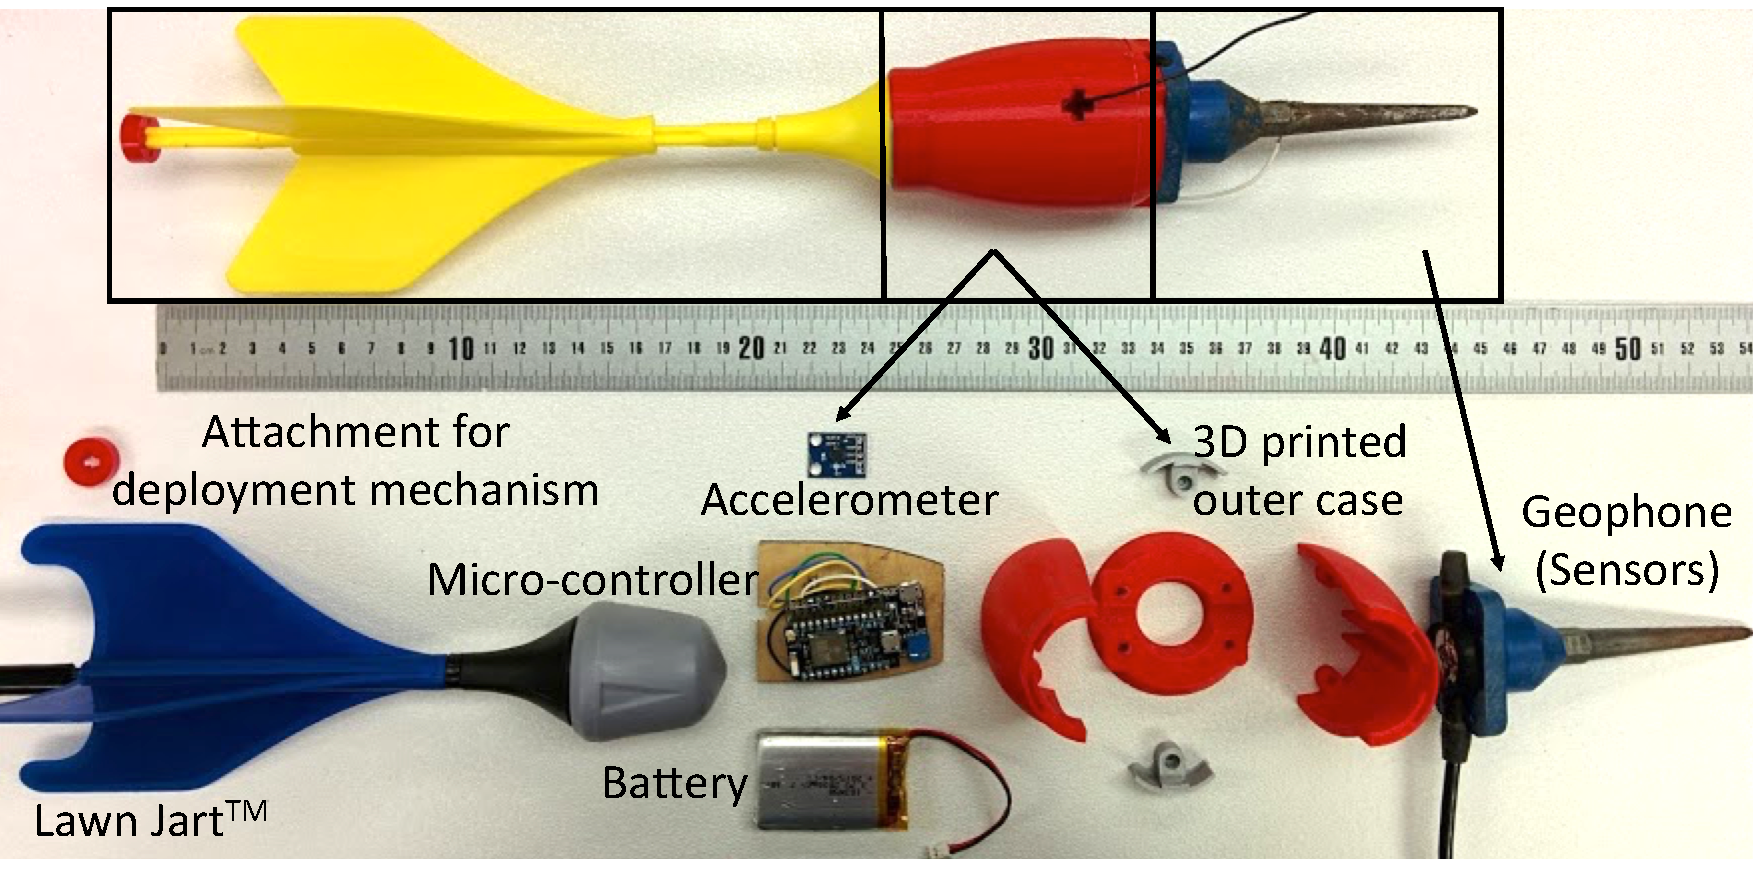
\includegraphics[width=\columnwidth]{Smart_Dart_overview.pdf}}
\caption{Components of the SeismicDart sensor: a lawn  Jart\textsuperscript{TM} fin, particle.io Photon\textsuperscript{TM}  micro-controller, 3D printed protective casing, and a geophone.} 
\label{fig:Smart_Dart_overview}
\end{figure}

%%%%%%%%%%%%%%%%%%%%%%%%%%%%%%%%%%%%%%% 
\subsection{Experiments} 
The following sections compare SeismicDart performance.
\subsubsection{ Drop tests in different soils}  


Proper planting of a geophone requires good contact with the soil and the geophone to be in a vertical position. 
Geophone protocol classifies a geophone as well planted if the angle of deviation is less than 10$^\circ$ and the spike has at least 40 mm of penetration.

To determine how SeismicDarts perform in different soils, this experiment measured penetration depth and angle of deviation in seven different soil types as a function of drop height. 
 The soil types were categorized by their compression strength, in kg/cm$^2$, measured using a soil pocket penetrometer (CertifiedMTP). Measurements for compression strength vary with small deviation in measurement location, so we repeated this measurement 10 times at 10 different locations in each soil type and computed the average.
 
 Experiments were conducted using the Seismic UAV to autonomously drop a payload of four SeismicDarts at a desired drop height. 
 Tests were conducted at drop heights of 10, 15, 20, and 25 m. 
 We measured angle of deviation and penetration depth for each drop.
 The angular deviation was recorded using two protractors.
 To measure penetration depth, the buried darts were marked where the spike met the soil, the dart was then pulled from the soil, and the distance from the spike tip to the marking was measured with calipers. 
  We repeated this measurement 12 times for each soil type at each drop height.  The soil compression strengths in these experiments ranged from 0.056 kg/cm$^2$ for river sand, to 4 kg/cm$^2$ for a hard-packed soccer field.

The four soil types with the lowest soil compression strength could be well-planted with low drop heights, so these tests were performed manually.
   Testing was performed by holding a dart at the tip opposite to the spike in a vertical position and releasing it at varying heights into 19 liter (5 gal.) buckets of soil. 

%Penetration depth and angular deviation were measured. %To measure penetration depth, the buried darts were marked where the spike met the soil, the dart was then pulled from the soil, and the distance from the spike tip to the marking was measured with calipers. The angular deviation was recorded using the accelerometer inside the dart.

 
  % These experiments shows that increasing drop height increases penetration on all soils tested.
  % Also, darts dropped in quiescent air remain vertical if they penetrate the soil.
Experiment results plotting penetration depth as a function of drop height are displayed in Fig.~\ref{fig:DepthPlotIndoors}, and angle of deviation as a function of drop height in Fig.~\ref{fig:AnglePlotIndoors}.   Both graphs are annotated with values for soil compression strength. 

\begin{figure} \centering
{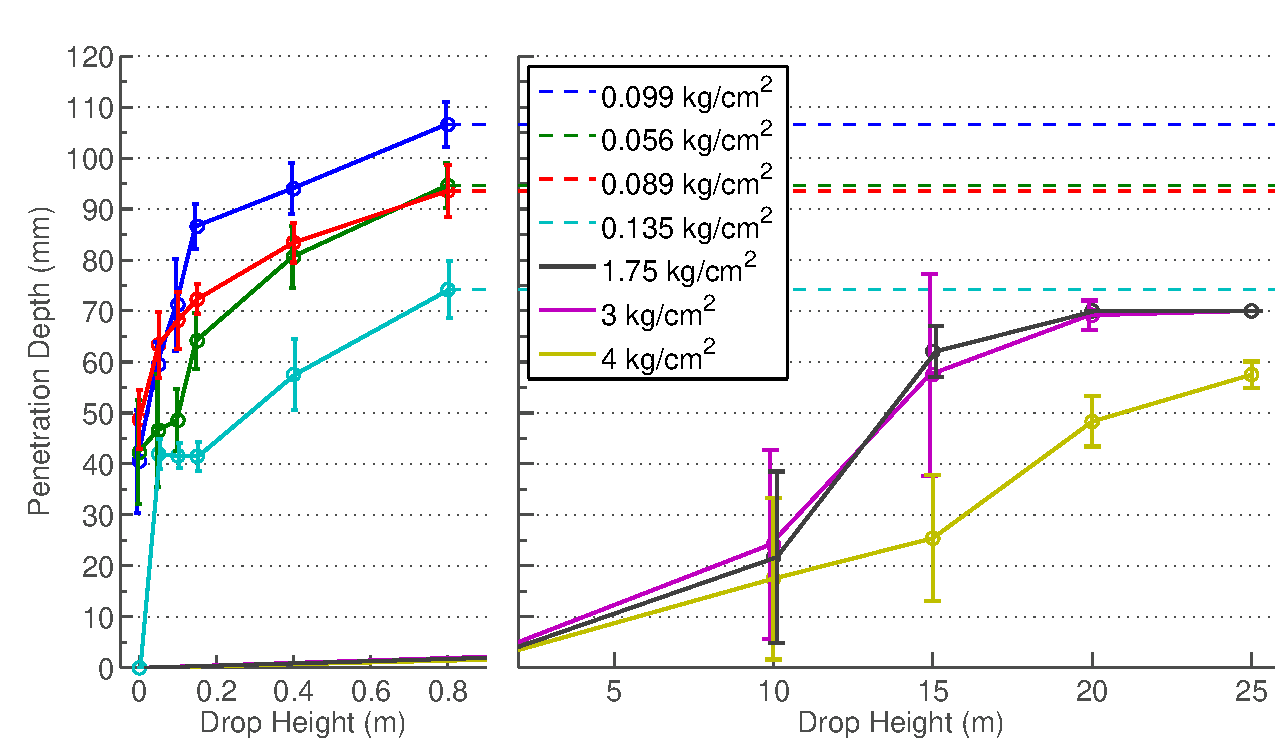
\includegraphics[width=\columnwidth]{AutoPenetrationDepth.pdf}}
\caption{Drop height vs. penetration depth in seven soil types. Drops were performed autonomously and each data point represents 12 trials. Increasing the drop height increased the penetration depth for all seven soil types.} 
\label{fig:DepthPlotIndoors}
\end{figure}

\begin{figure} \centering
{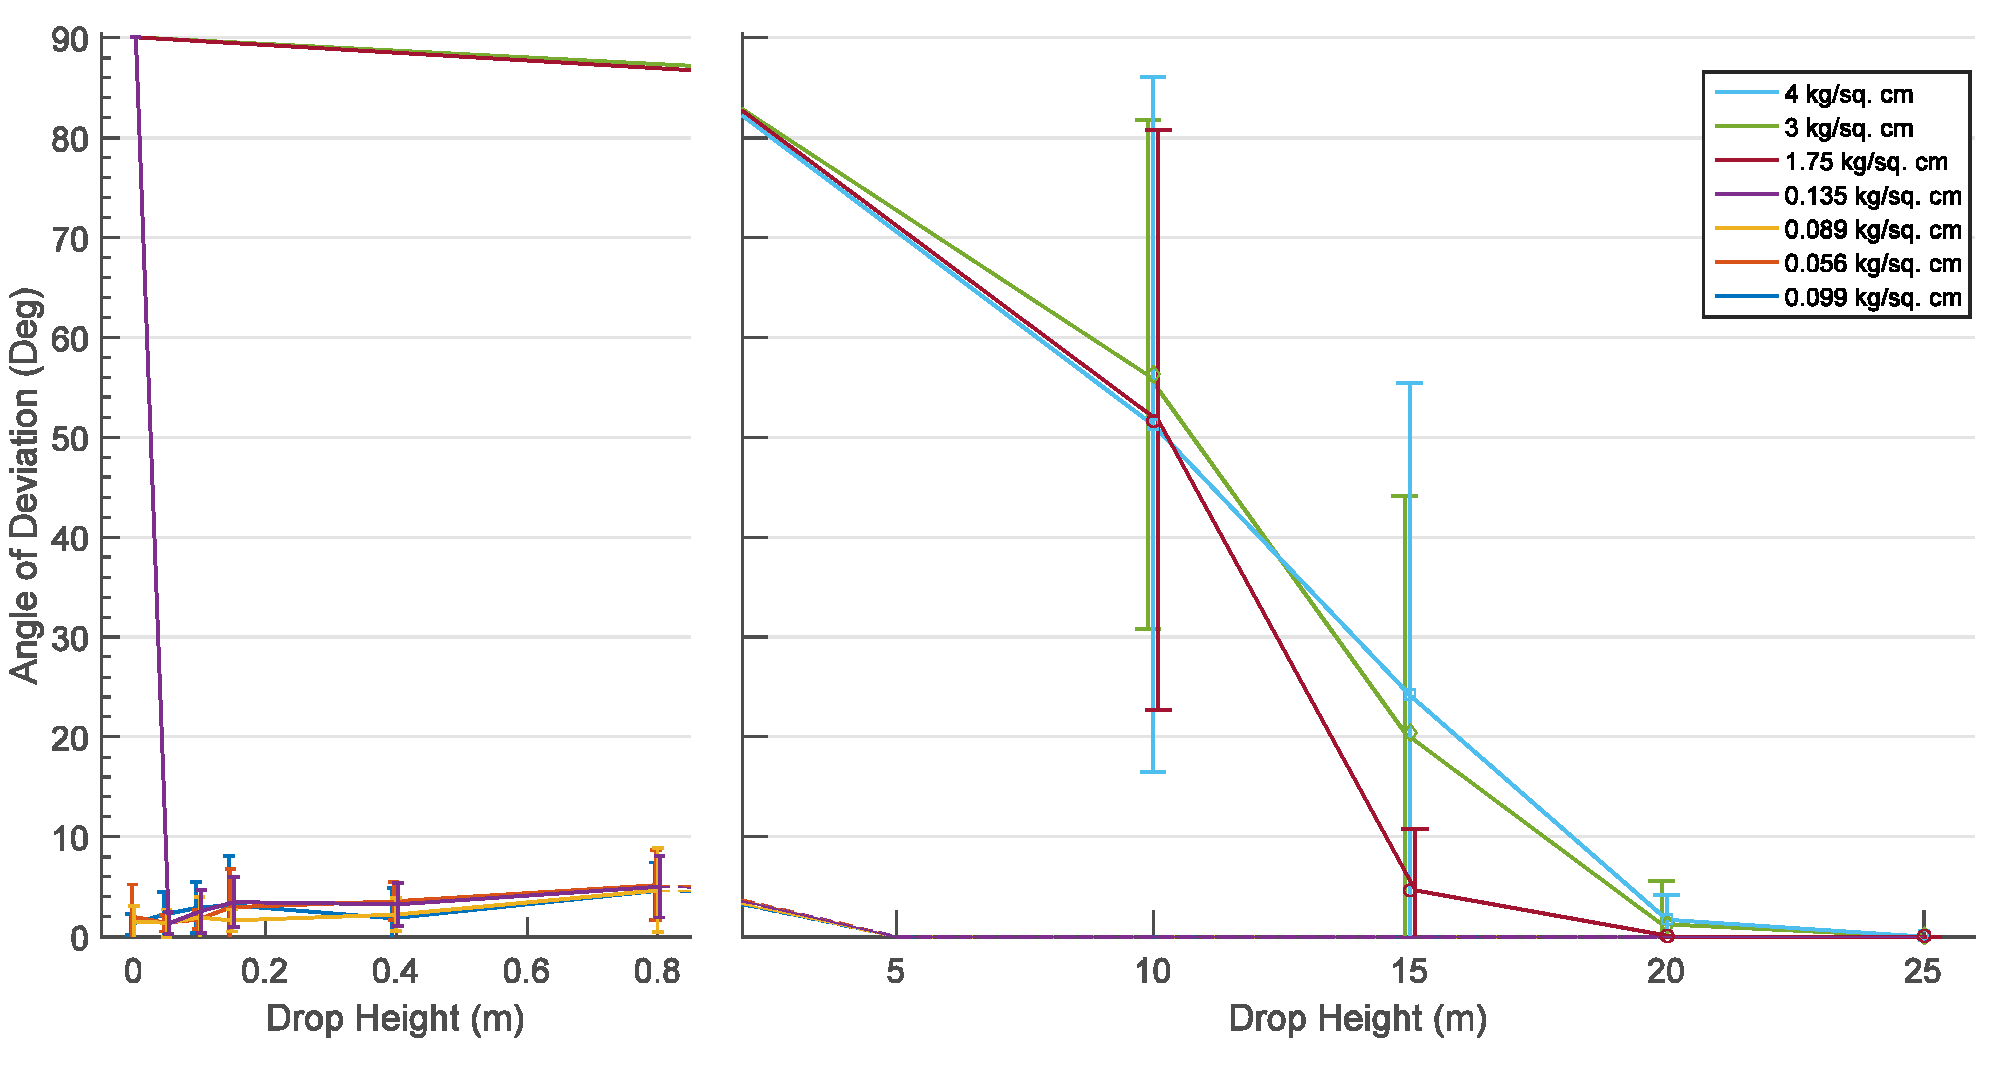
\includegraphics[width=\columnwidth]{AutoPenetrationAngle.pdf}}
\caption{Drop height vs. angle of deviation in seven soil types. Drops were performed autonomously and each data point represents 12 trials. Increasing the drop height reduced the angle of deviation for all seven soil types.} 
\label{fig:AnglePlotIndoors}
\vspace{-1em}
\end{figure}

If a SeismicDart is dropped from a sufficient height into penetrable soil, the spike will be buried into the soil, and the geophone will have small angular deviation from vertical. Soils with higher compression strength require higher drop heights. Error bars show that variance decreases with drop height for both angle of deviation and penetration depth.  
 All drops from heights 20 m or more achieved the goals of an angle of deviation less than 10$^\circ$ and a penetration at least 40 mm of penetration.   

The autonomous tests were conducted with 16 km/hr winds, demonstrating that drop heights 20 m or higher were sufficient to counter disturbances from wind. %https://www.windfinder.com/forecast/galveston_airport





%\subsubsection{Straight vs.\ Twisted Fins}

%To determine the difference in performance between SeismicDarts with straight fins and twisted fins, we ran a drop test with 10 trials for both types of dart at a constant height in one soil type. Each trial was initialized by holding the dart horizontally at a height of 9.8 meters, dropping it into the soil, and recording the penetration depth and angular deviation. Holding the darts horizontally emphasized the angle-correcting behavior of the fins. The penetration depth and angular penetration were measured and recorded as in the previous experiment. A graph showing the values recorded for penetration depth and angular deviation in Fig.~\ref{fig:StraightBentDepth}  reveals that SeismicDarts with twisted fins had less angular deviation, but also less penetration depth. 

%\begin{figure} \centering
 % {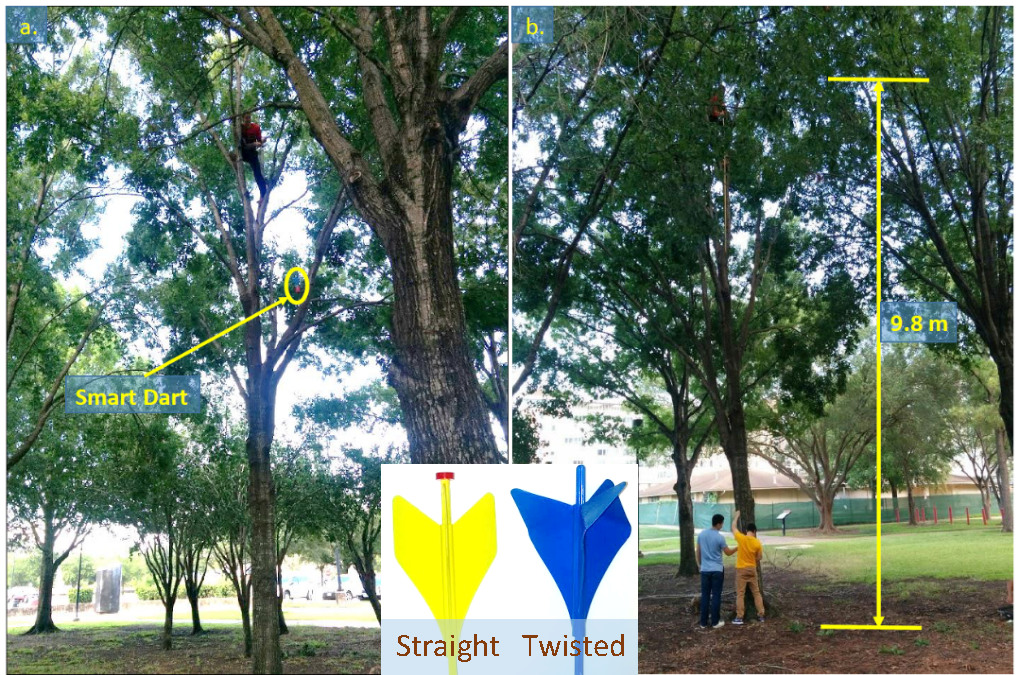
\includegraphics[width=\columnwidth]{StraightvsBent_pic.pdf}}
 %\caption{Outdoor drop test comparing straight vs.\ twisted fins performance:
 %a.)  dropping a SeismicDart,  
% b.)  measuring drop height.} 
% \label{fig:StraightBentPic}
 %\vspace{-1em}
%\end{figure}
%\begin{figure} \centering
%  {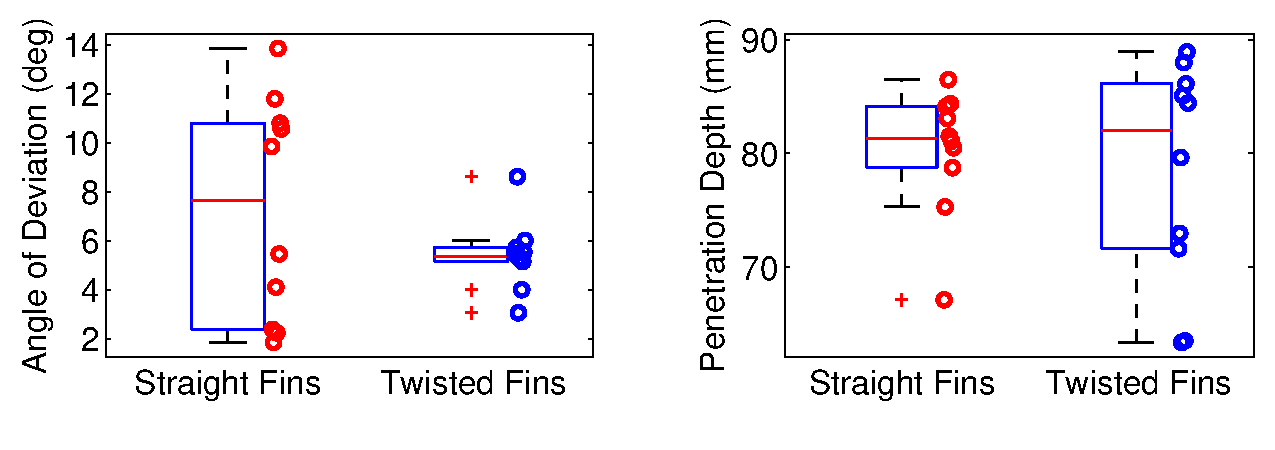
\includegraphics[width=\columnwidth]{StraightvsTwistedAngleDepth.pdf}}
% \caption{\label{fig:StraightBentDepth}Straight vs.\ twisted fins comparing a.) penetration depth b.) angle of deviation. Experiment used a fixed drop height of 9.8 m.} 
%\end{figure}

%\begin{figure}\centering 
%\subfigure[\label{subfig:StraightBentDepth}]
%  {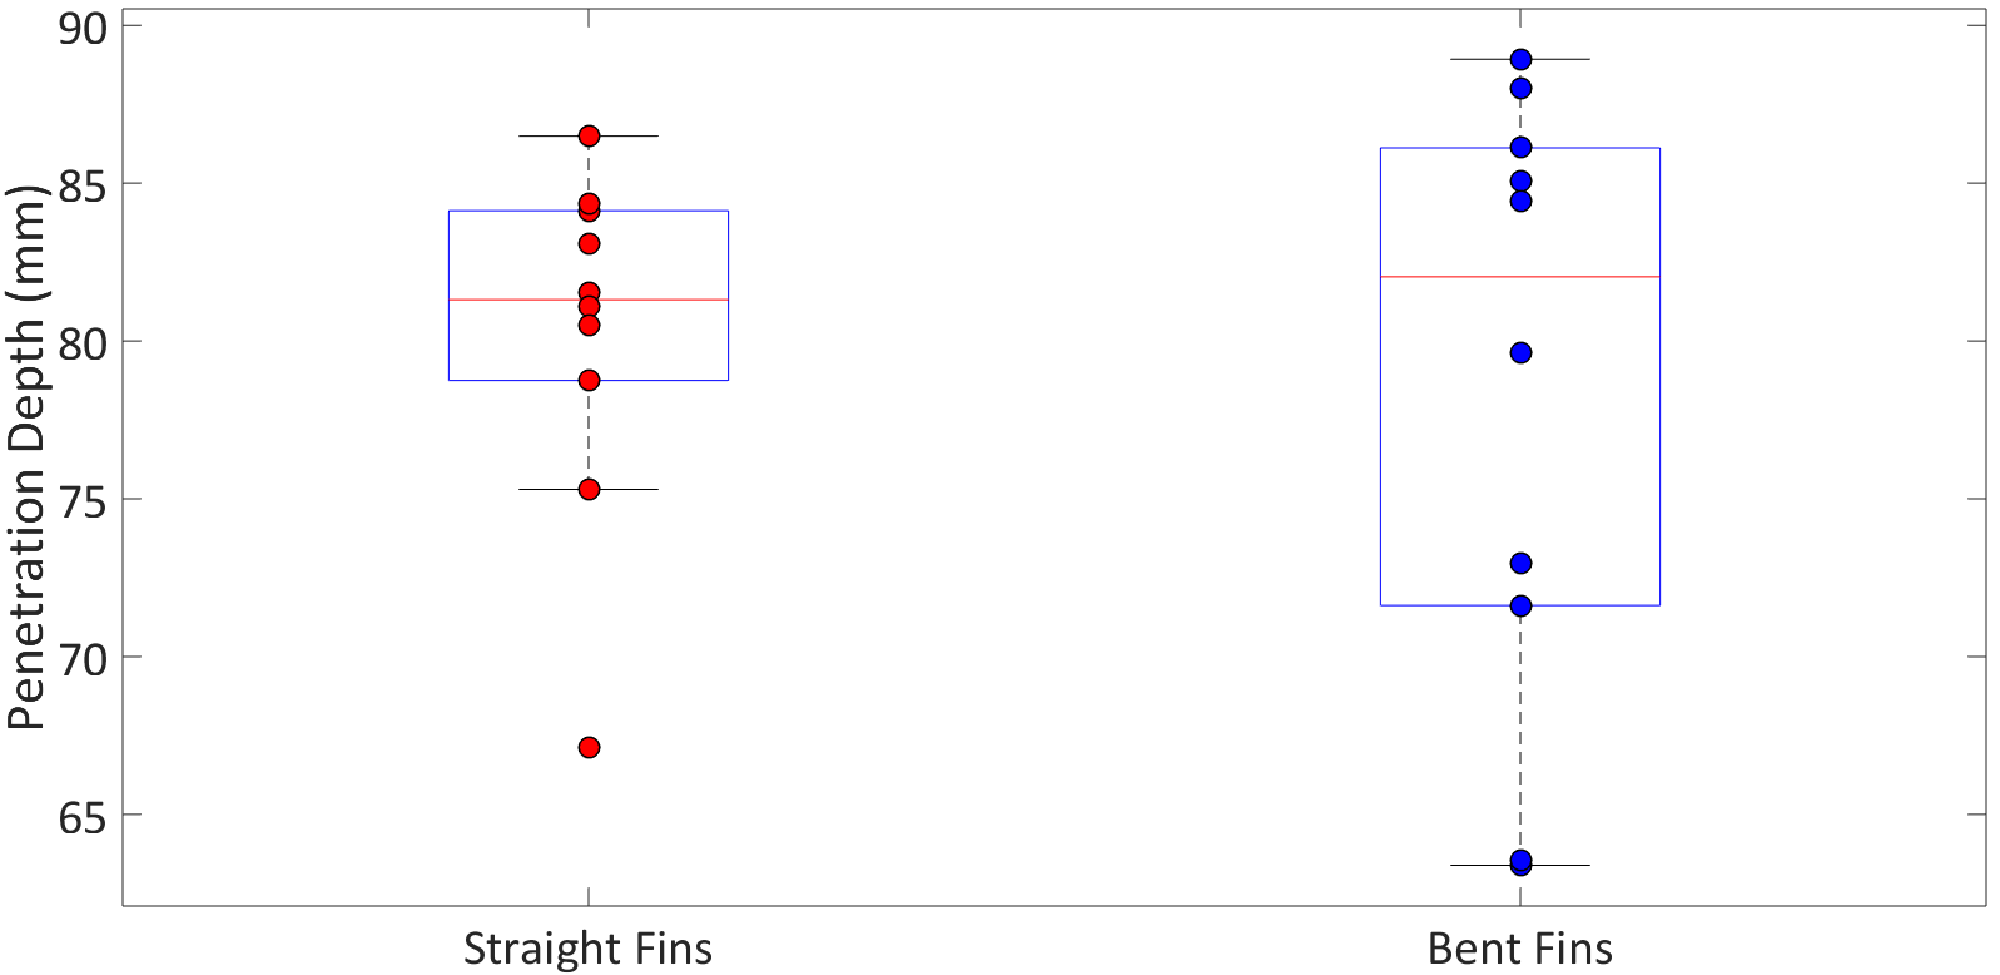
\includegraphics[width=.45\columnwidth]{StraightvsBent_depth.pdf}}
% \subfigure[\label{subfig:StraightBentAngle}]
%  {\includegraphics[width=.45\columnwidth]%{StraightvsBent_angle.pdf}}
%   \vspace*{-.1in}
 %\caption{Straight vs Bent fins comparing a.) Penetration Depth b.) Angle of Deviation. Experiment used a fixed drop height of 9.8 m. \label{fig:StraightBent}}
 %\vspace*{-.1in} 
%\end{figure} 
\subsubsection{Shot gather comparison} 
Geophysical explorationists often use thousands of geophones to conduct a seismic survey. 
 As a proof-of-concept, this experiment ran a small-scale seismic survey to compare the performance of a traditional cabled four geophone system with readings from four autonomously deployed SeismicDarts.
Flying autonomously at a drop height of 25 m, the Seismic UAV flew to GPS waypoints spaced 4 m apart and deployed one dart at each location. 
A seismic survey technician manually planted four traditional cabled geophones, each 10 cm from a deployed SeismicDart. 
A seismic wave was generated using a sledge hammer hitting a steel plate.

Results of the field test comparison between the traditional cabled geophone system and the SeismicDarts are shown in Fig.~\ref{fig:shotgather_auto_drop}.   
Data were obtained using a \emph{Strata-Visor}, a device that can obtain, store, and plot the sensed data. 
The \emph{Strata-Visor} is extensively used with traditional geophone setups because the geophones can only sense vibrational waves and are dependent on other devices for storage and data processing. 
To allow a fair comparison, the SeismicDart's  ability to store sensed data was not used in this experiment. 
 The \emph{Strata-Visor} records the geophone voltage at 2000 Hz, using an 24 bit ADC.

The readings from both systems are qualitatively similar, with no discernible phase or amplitude differences. Let $X$ be measurements from the traditional geophone and $Y$ the corresponding voltages from a SmartDart.
The percent peak-to-peak error and normalized root-mean-square error (NRMSE) are defined as
\begin{align}
e_{pp} &= 100 \left( \frac{ \max(X) - \min(X) }{ \max(Y) - \min(Y) } -1\right) \\
  \text{NRMSE} &=\frac{100}{\max(X) - \min(X)} \sqrt{ \frac{ \sum_{i=1}^n \left( X_i - Y_i \right)}{n} }.
\end{align}
The peak-to-peak errors were [-6.33, -1.15, -1.81,  9.84] \% for sensors at [4,8,12,16] m from the source.
 The NRMSE were [1.05,1.27,3.98,4.39] \% for sensors at [4,8,12,16] m from the source.
%$e_{\text{4 m}}  =  -6.3 \%, e_{\text{8 m}}  =  11.93 \%, e_{\text{12 m}}  = -1.81\%, e_{\text{16 m}}  = 0.981 \%$. 
%The RMSD error were $RMSD_{\text{4 m}}  =  -6.3 \%, RMSD_{\text{8 m}}  =  11.93 \%, RMSD_{\text{12 m}}  = \%, RMSD_{\text{16 m}}  = 0.981 \%$. 
Readings were also compared using a Pearson product-moment correlation coefficient, which gives a correlation measurement between $-1$ and $+1$ where $+1$ is total positive linear correlation.
\begin{align}
\rho_{X,Y} = \frac{E\left[  (X-\mu_X) (Y-\mu_Y)  \right]}{  \sigma_X, \sigma_Y}
\end{align}

The correlation coefficients were $\rho_{\text{4 m}}  =  0.9813, \rho_{\text{8 m}}  =  0.9836, \rho_{\text{12 m}}  =  0.8600, \rho_{\text{16 m}}  = 0.8114$. These correlations decrease with distance. The SeismicDart is subject to low-amplitude noise, which is easiest to see in the fourth sensor because it was 16 m from the seismic source and thus had the lowest signal amplitude.  This noise is potentially due to wind striking the SeismicDart's fin. The effect of noise can be mitigated by using larger seismic sources such as a vibration truck or explosives.



\begin{figure} \centering
  {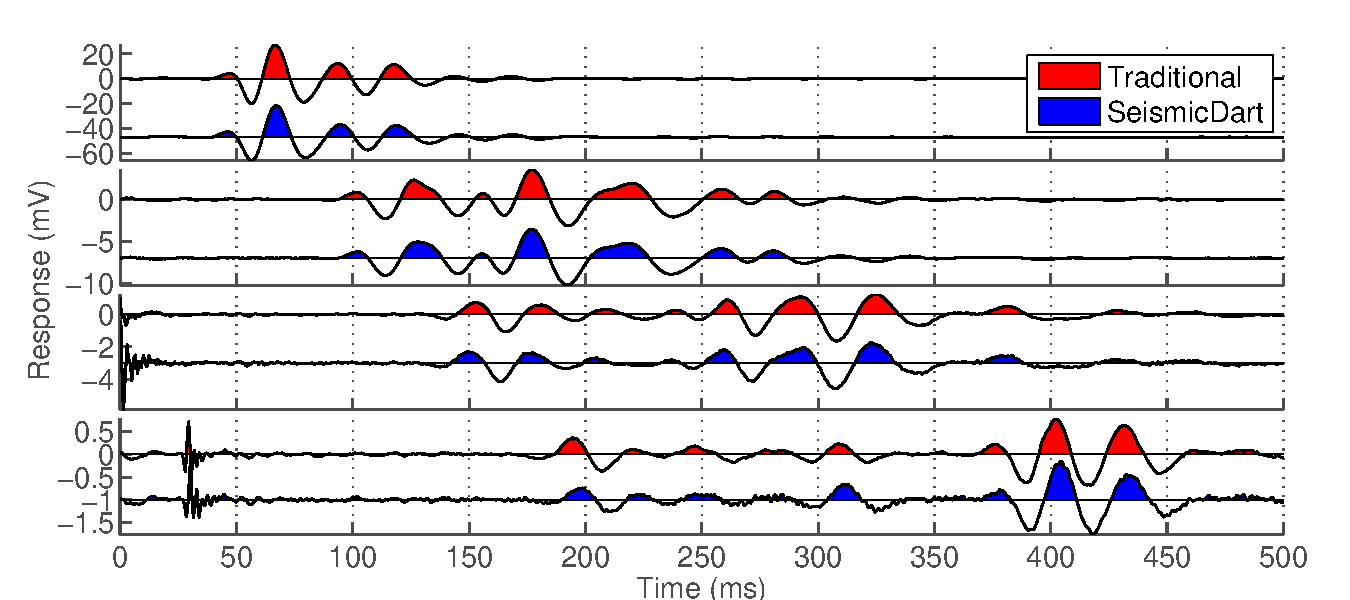
\includegraphics[width=\columnwidth]{SeismicSurveyComparison.pdf}}
 \caption{Raw voltage data from shot gather comparison of four traditional geophones and four autonomously dropped SeismicDart sensors.  
 \label{fig:shotgather_auto_drop}}
\end{figure}

\subsection{SeismicDart Deployment and Retrieval}
First the SeismicDarts are loaded onto to a UAV. 
Currently a maximum of four sensors can be dropped in a single flight. 
The flight plan communicated to the UAV provides a GPS waypoint for each SmartDart. 
The UAV flies to and drops a SmartDart at each waypoint, then returns home. 

Deployment is only one part of a survey. Large surveys require moving and reusing sensors.  
Because SmartDarts are more expensive than standard geophones, rapid reuse is essential.
The UAV has an underslung hook for picking up a SeismicDart.
Retrieval is facilitated by attaching a wire loop to the SeismicDart tail, which provide a target 300 mm in diameter for the hook.
Currently retrieval is performed by manually piloting the UAV, but this level of accuracy is within the accuracy of UAVS equipped with RTK GPS.
Automating retrieval is out of the scope of this paper.
Fig.~\ref{fig:SeismicDart_DR} shows a SeismicDart being retrieved and redeployed.


\begin{figure} \centering
  {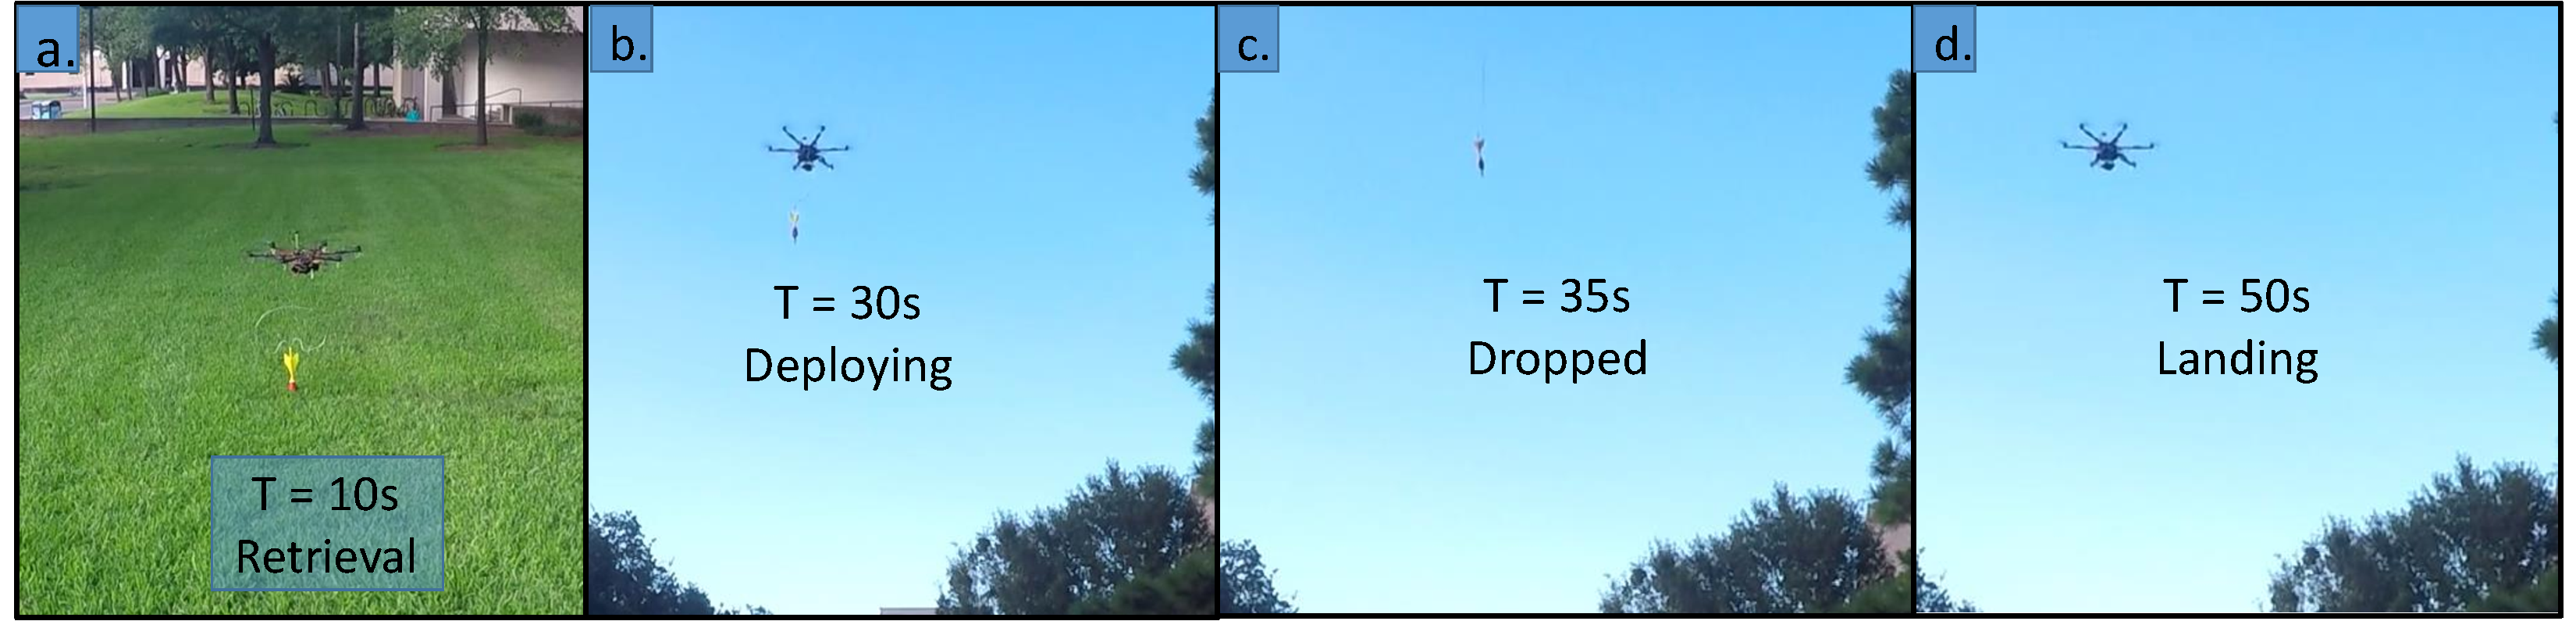
\includegraphics[width=\columnwidth]{SeismicDart_DR.pdf}}
 \caption{SmartDart retrieval and redeployment.  See video attachment. 
 \label{fig:SeismicDart_DR}}
\end{figure}
 
%
\section{SeismicSpider}\label{sec:SeismicSpider}

Traditional geophones are mounted in an insulated shock resistive enclosure on a spike. The spikes, varying in length, are inserted into the ground to ensure a firm coupling with the environment. The design of our Seismic Spider prevents full depth insertion of the three inch spikes. 

	To overcome the coupling issue we are using three geophones per station compared to the typical one. Our immediate goals are to compare amplitude and phase response to that of a standard single station.	

\begin{figure} \centering
  {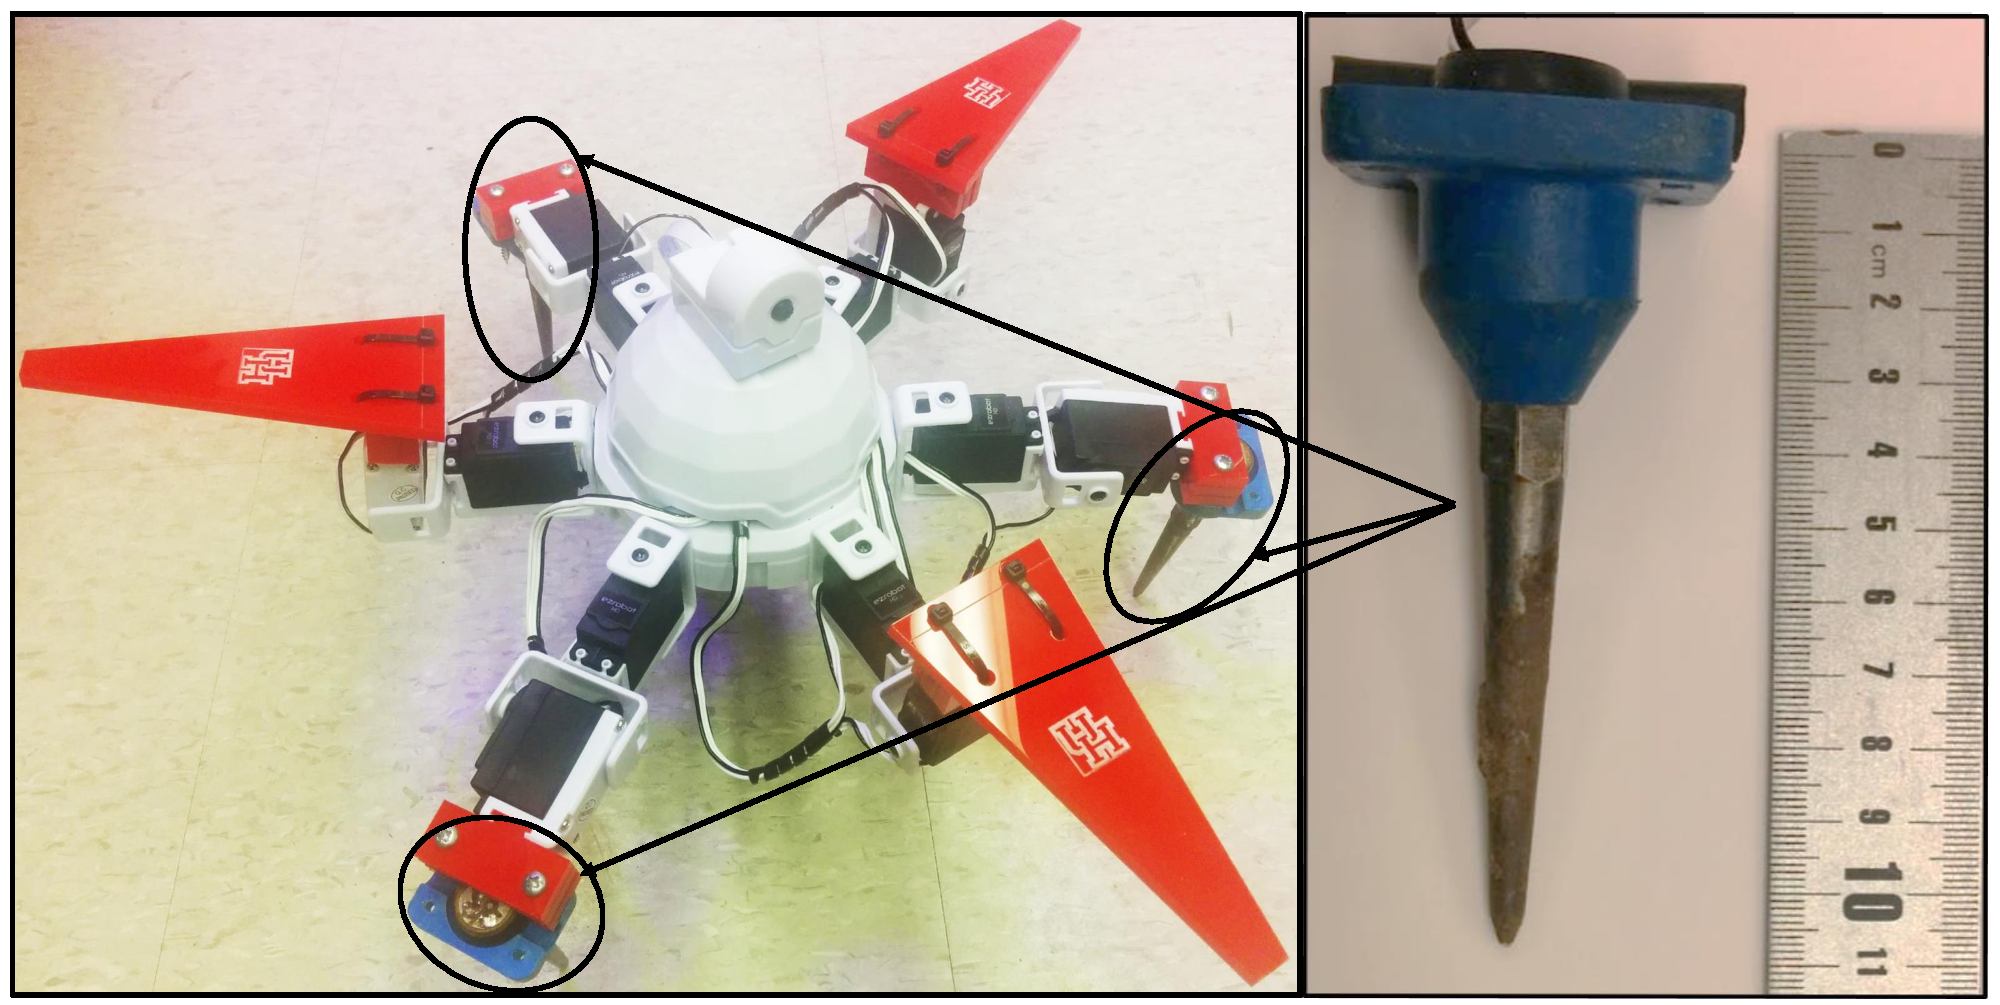
\includegraphics[width=\columnwidth]{Hex_overview.pdf}}
 \caption{The SeismicSpider is a six-legged mobile robot where three legs are replaced by geophones. It senses and records seismic data.} 
 \label{fig:TradvsAutoDrop}
\end{figure}
\subsection{Design}

The Seismic Spider is built from the Six Hexapod kit designed by EZ Robots. Each of the six legs are powered by two 15 kg/cm lever servos. The peg legs were replace by three GS-20DM 14 Hz geophones from Geospace Technologies. The remaining three were designed to match the geophone dimensions and reflect UH school spirit.

 Our initial plan to use three geophones require the spider to raise the three inactive legs while acquiring data. This lack of support caused excessive strain on the three servo motors responsible for holding the spider upright introducing unwanted vibration into the system. We found positioning the geophone legs at 20o to normal enhanced the stability and relieved the excessive stress on the servos. With each planted geophone angled inward superposition creates one vertical geophone. The three geophones were in series.

\subsection{Experiments}
\subsubsection{Exp 1: Accuracy plot}
Hexapod move to desired GPS location  (plot accuracy)\\
\subsubsection{Exp 2: Shot gather comparison}

A line of twenty four geophones, GS-20DM 14 Hz, were laid out at one meter intervals with our inline source seven meters from the nearest geophone. Beginning from the farthest offset of 31 meters we manually aligned the Spider with the corresponding geophone, fired the source, then moved one meter ahead. 

\paragraph{Results}
Data from the shot gather comparison is shown in Fig.~\ref{fig:shotgatherHexpod}.
We found a correlation, unmeasured, with the standard geophones and we more than compensated for loss of amplitude with three geophones, the response was 5 dB greater that the single geophone. The geophone wires proved insufficient to insulate against 60 Hz. Due to the small amount of usable data we were not able to gain meaningful results for phase analysis.   

\begin{figure} \centering
  {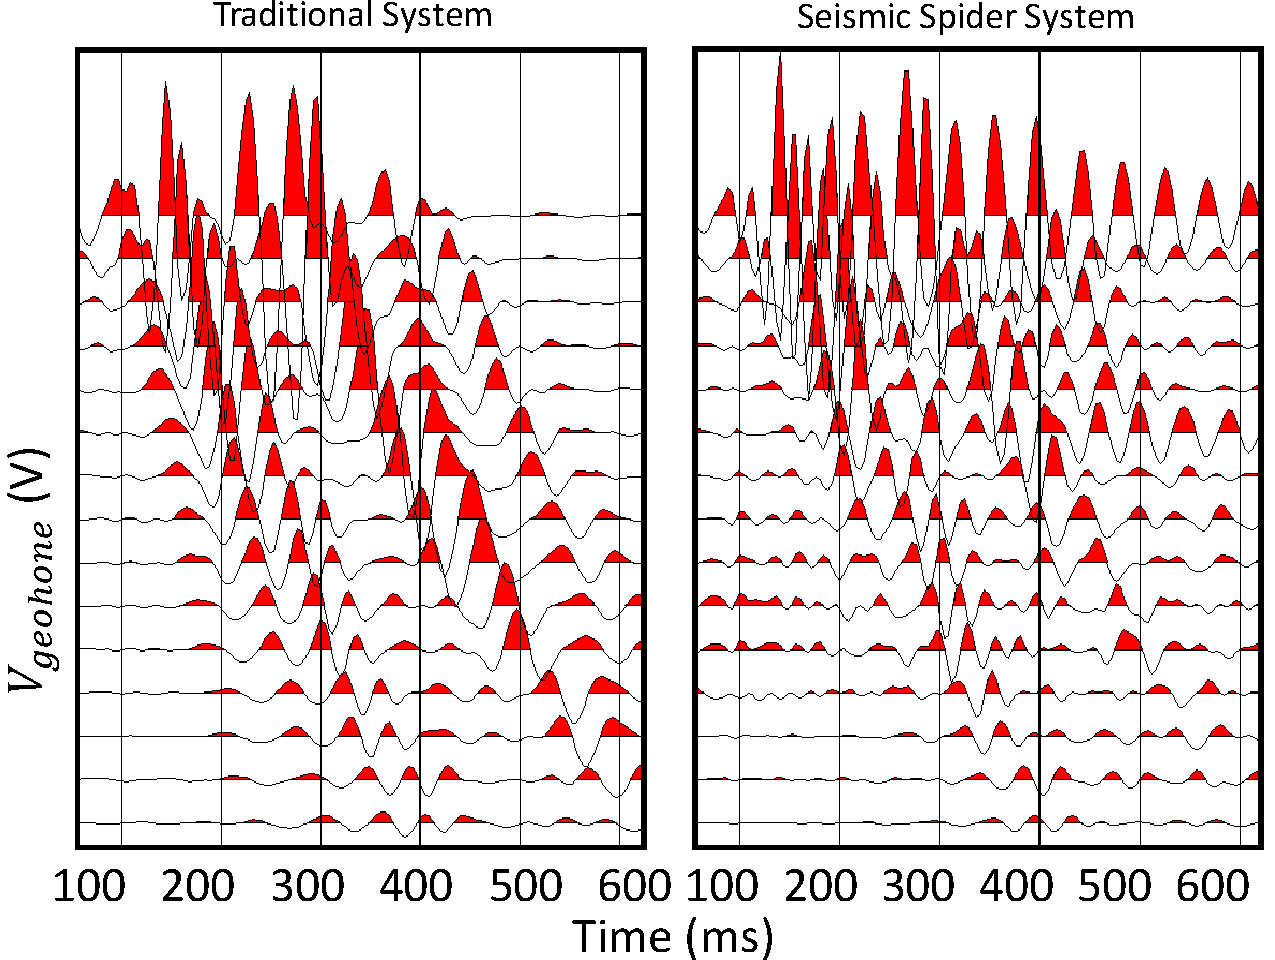
\includegraphics[width=\columnwidth]{shotgather_hex.pdf}}
 \caption{Shot gather comparison of traditional geophones vs. hexapod sensor. 
 \label{fig:shotgatherHexpod}}
\end{figure}


\paragraph{Future work}	we must filter 60 Hz noise, compare adding geophones to all six legs, and design a larger seismic survey to ensure adequate data for phase analysis.   

\subsubsection{Exp 3: Deploying and Retrieving Hexapod}
\todobox{describe piloting the drone for retrieval.  Need image}
%
\section{UAV and deployment unit}\label{sec:DeploymentUnit(UAV)}

\subsection{Design}
The UAV is a custom-built, 177 cm wing span hexacopter, controlled by the Pixhawk flight controller running ArduPilot Mega flight software. The UAV has a 3DR GPS module using the UBlox NEO-7 chipset.


 The SmartDart deployment mechanism allows the UAV to carry four Smart Darts in a circular array, and release them when it reaches the desired GPS location, one at a time, as shown in Fig.~\ref{fig:deployment_system}.
 The rear of the dart has a circular tip that locks into the deployment mechanism, and rests on a rectangular slot-path. 
 A servomotor rotates the dart tips through the rectangular slot-path, allowing darts to release from a circular opening.



\begin{figure} \centering
  {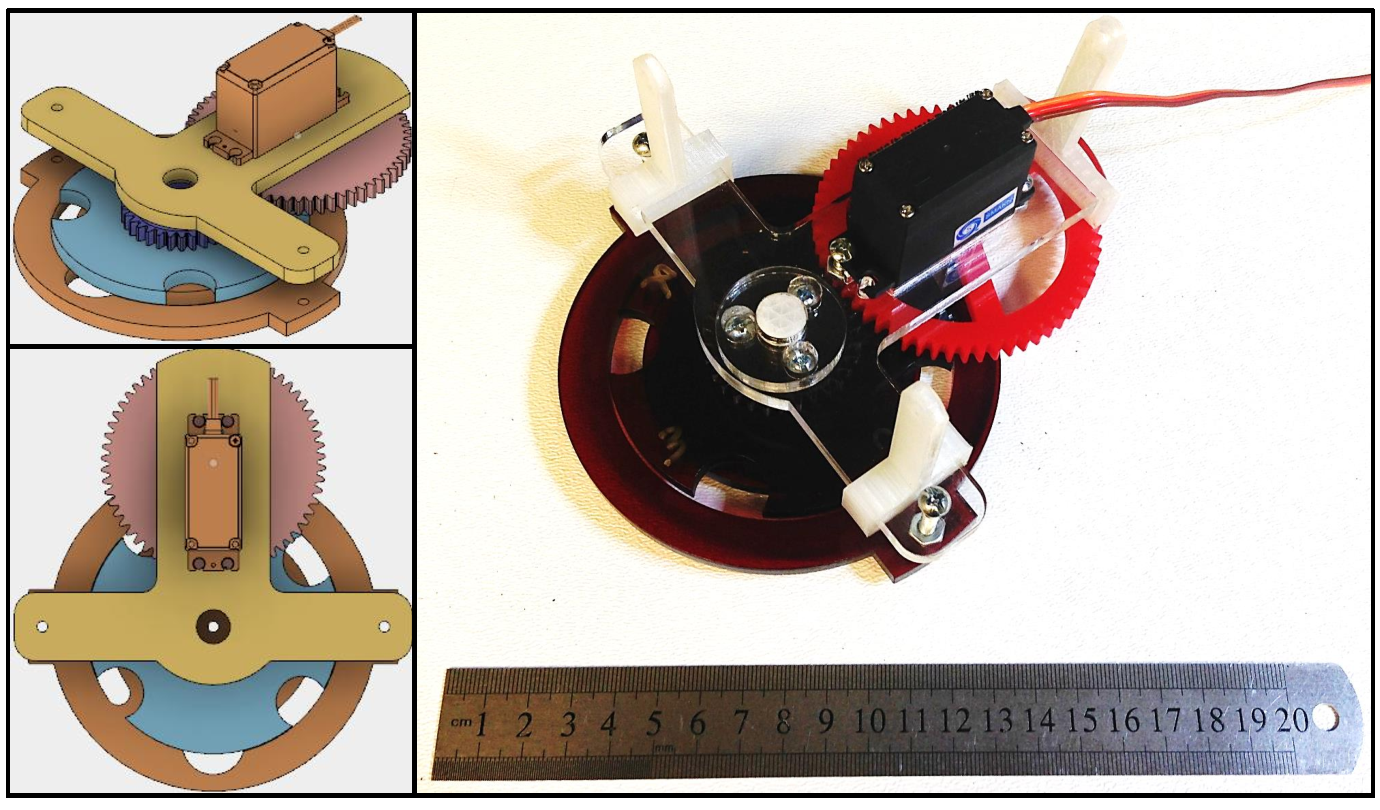
\includegraphics[width=\columnwidth]{deployment_system.pdf}}
 \caption{Deployment system for dropping SmartDarts from the UAV. Pictured design holds 4 darts, but can be scaled according to the UAV's carrying capacity.} 
 \label{fig:deployment_system}
\end{figure}



\subsection{Experiment}


\subsubsection{Autonomous drop demonstration and accuracy}

The current drone can place the SmartDart within $\pm1$ m of the desired location.  
This range is within tolerances for seismic surveys because
(1) there are often features (rocks, water, etc.) that require this amount of error from theoretically assigned locations,
(2) some survey designs include a random placement component to improve noise cancellation,
(3) this error minimally perturbs  the data since seismic waves travel at 600 m/s in near surface, so a one-meter inaccuracy equates to $\approx$1.6 ms delay,
(4) the response of a receiver to seismic vibrations is an average over a number of meters.

The critical factor is to know within 10 cm accuracy the geophone location.  Such accuracy can be obtained thorugh Real Time Kinematic GPS systems. Knowledge of the exact location allows corrections for jitter in signal arrival times due to  placement inaccuracy.


%Exp 4: Automatic drop from drone, accuracy in placement
\textbf{\begin{figure} \centering
  {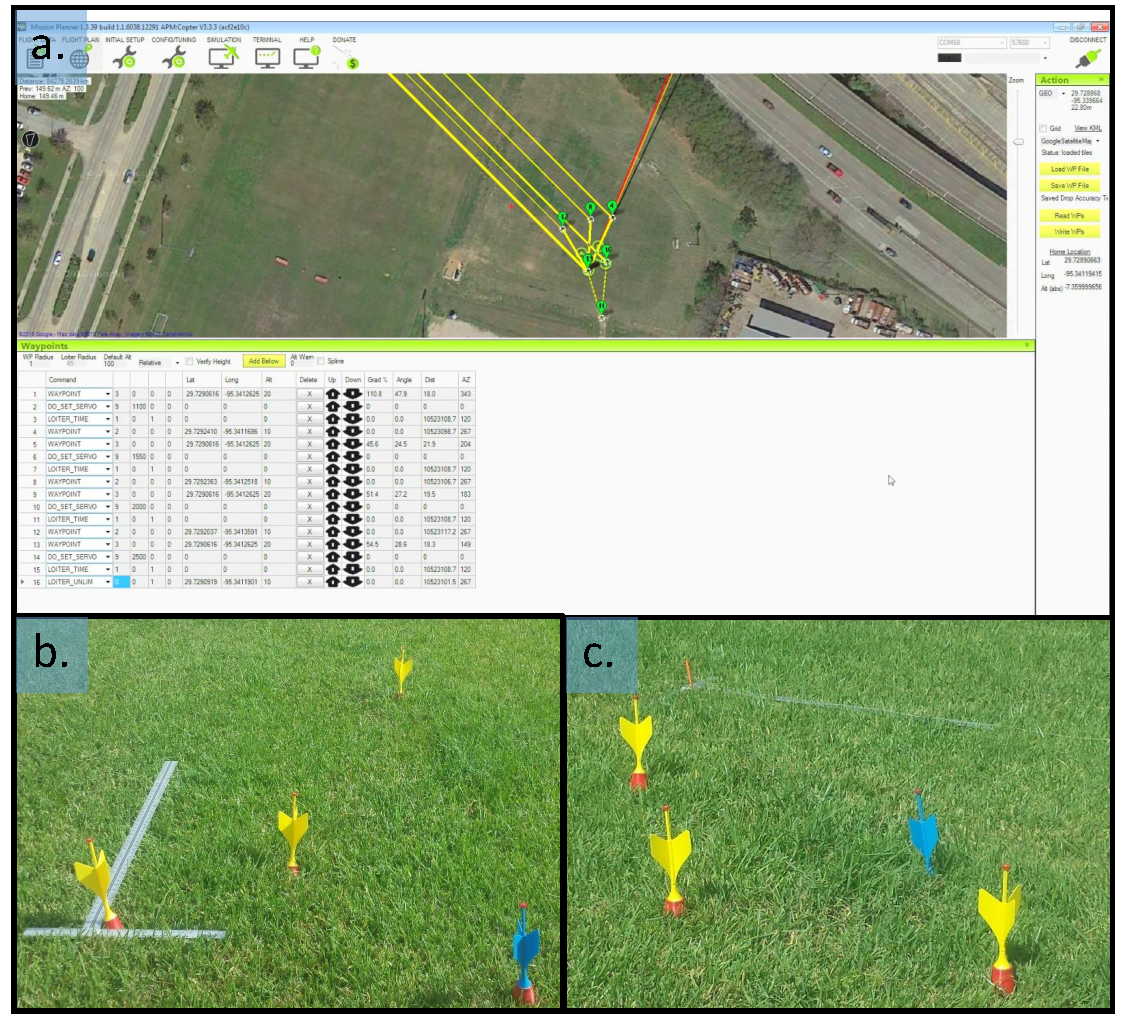
\includegraphics[width=\columnwidth]{accuracy_test_overview.pdf}}
 \caption{a.) Flight plan of accuracy test b.) First set of dart with reference axes c.) Third dart set } 
 \label{fig:Accu_test_darts}
\end{figure}}

For the accuracy test, 6 sets of darts, 4 darts in each set, were dropped on the same GPS waypoint. Between each drop, the UAV travelled to a nearby GPS waypoint to cancel out the flight controller's stable hover.  This path is shown in Fig.~\ref{fig:Accu_test_darts}a. The UAV returned to the launch platform to be reloaded and data was recorded after each set.

To record data, one dart was picked from the first set as the reference point (the lower left in Fig.~\ref{fig:Accu_test_darts}b), hence the first data point will be (0,0). A 1-m T-square was placed with the origin at the dart's drop point to establish the axes.

After the first set of data was been recorded, the darts were collected and reloaded on the UAV for the next deployment set.
 A rod was placed in the position of the first dart to keep reference as shown in Fig.~\ref{fig:Accu_test_darts}c. 
 The T-square was kept in place and mason twine was suspended to lengthen the reference axes. 
 Future deployment were measured  using the reference point and axes.


\subsubsection{Height vs. penetration depth}
%Exp 5: Height vs. penetration depth

FAA rules require that UAVs fly below 400 feet (122 m). Our highest drop tests were from 20 m, and resulted in well-planted geophones on a grass field with density 3.3 kg/cm$^3$. Harder soils may require faster impact velocity, so this section examines possible impact velocities as a function of drop height.
For ease of analysis we will assume the SmartDart has a constant coefficient of drag $C_d$ and that the drag force is proportional to velocity squared and equal to $\frac{1}{2} v^2 \rho A C_d$, where $v$ is the velocity, $A$ the cross-sectional area and $\rho$ the density of air.  The tests were performed near sea level, so $\rho \approx 1.225  \text{kg/m}^3$ and the dart body is 0.06 m in diameter so $A=0.028$ m$^2$.  We will assume the dart $C_d$ is between that of a streamlined body $C_d=0.04$ and that of an arrow $C_d=1.5$~\cite{miyazaki2013aerodynamic}, and choose that of a sphere $C_d=0.47$.
The terminal velocity is 
\begin{align}
v_T = \sqrt{\frac{2 m g}{\rho A  C_d}} \approx 59 \text{m/s}
\end{align}
The velocity at impact is a function of the drop height $h$.
\begin{align}
v_{impact} = v_T  \sqrt{ 1 - e^{ -\frac{\rho A  C_d}{m} h }} \approx 59\sqrt{ 1 - e^{ -0.008 h }} \text{m/s}
\end{align}
With  $C_d=0.47$, our drop from 20m achieves only 38\% the terminal velocity (19.0 m/s), and for $C_d=0.04$ only 12\% terminal velocity  (19.7 m/s).
%This implies our tests are far from the limits of the SmartDart's per
This implies the SmartDart is suitable even for much harder soils than tested this far.

%\begin{figure} \centering
%  {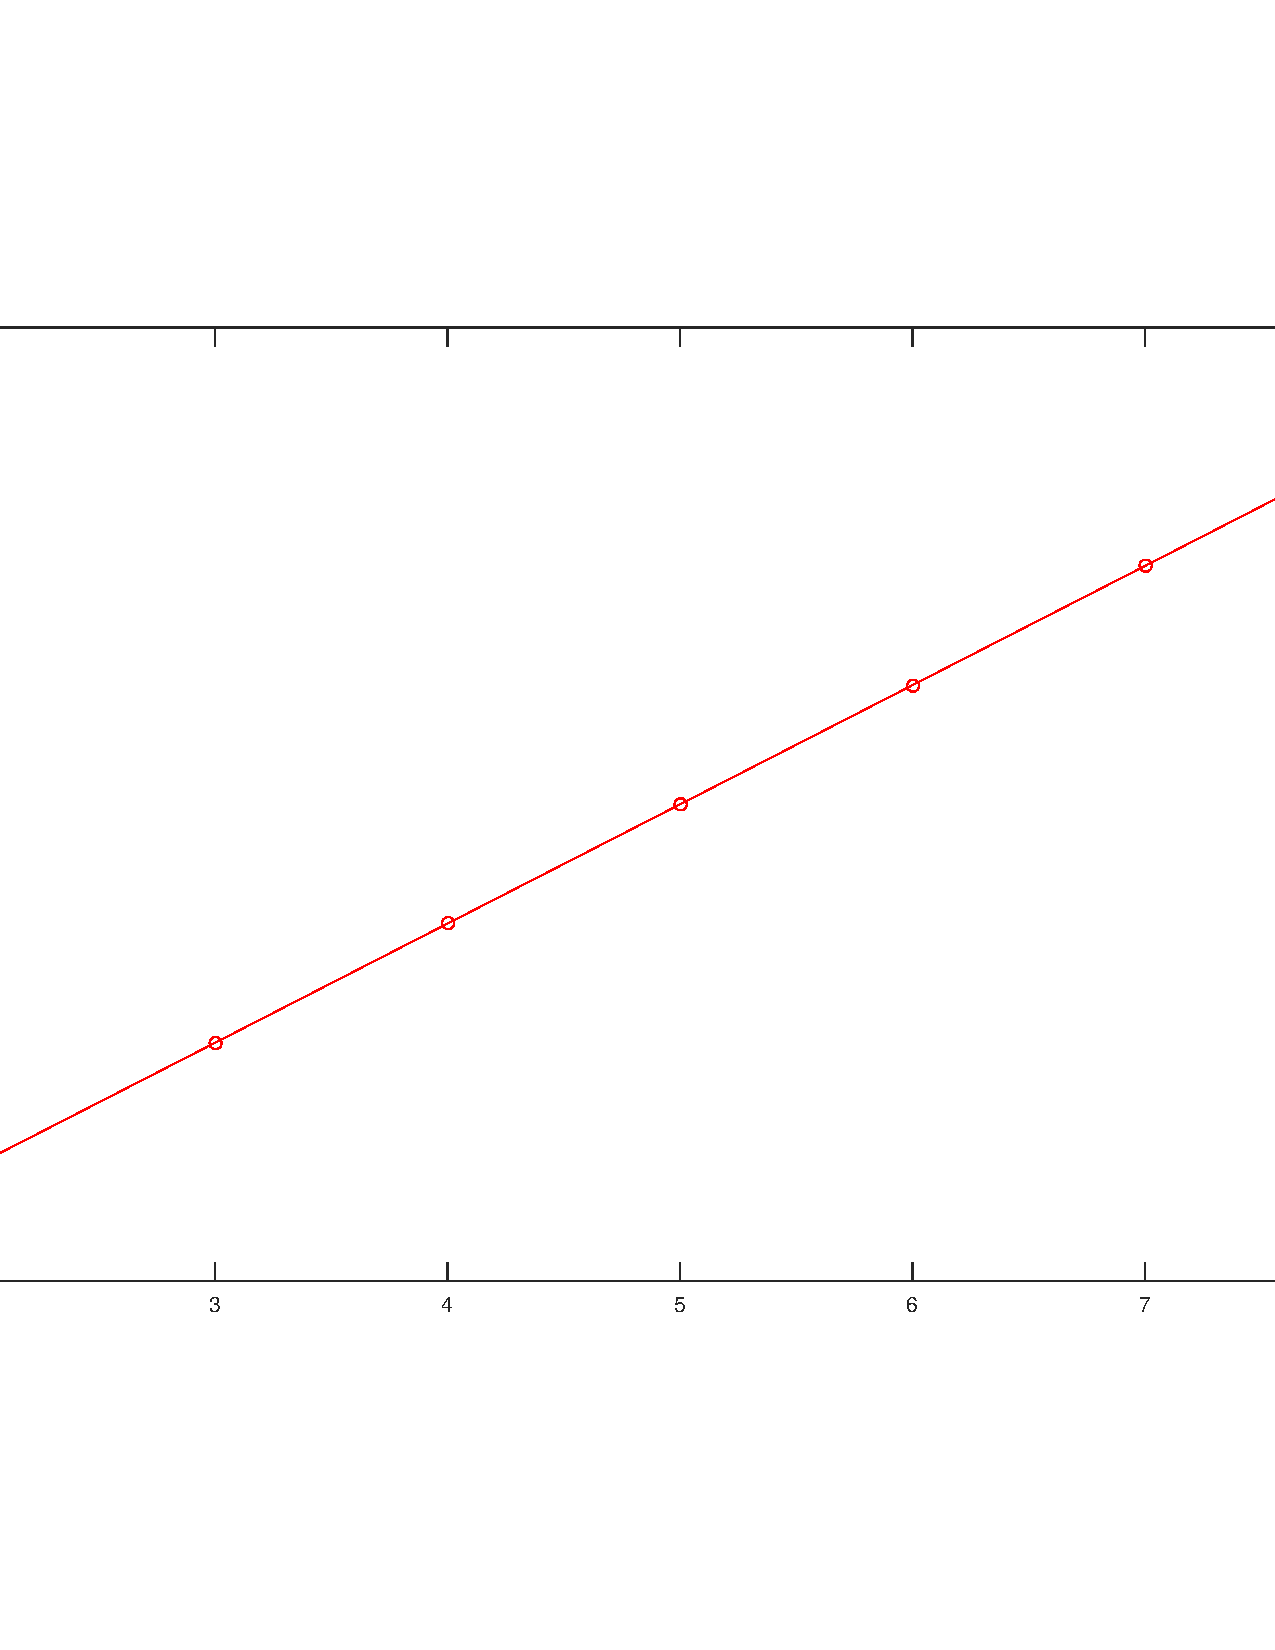
\includegraphics[width=\columnwidth]{replace_graph.pdf}}
% \caption{Plot of pneumatic cannon firing angle vs ending angle} 
% \label{fig:TradvsAutoDrop}
%\end{figure}

%
\section{Comparision}\label{sec:Comparision}


\begin{figure} \centering
  {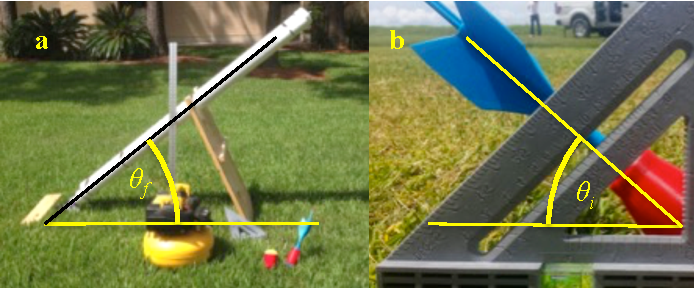
\includegraphics[width=\columnwidth]{CannonPicture}}
 \caption{A pneumatic launcher for SeismicDarts.  Ballistic dart deployment has limited usefulness because the incident angle is equal to the firing angle.} 
 \label{fig:CannonPicture}
\end{figure}

\begin{figure*}[htb]
\centering
\renewcommand{\figwid}{0.5\columnwidth}
\begin{overpic}[width =\figwid]{sim1_1.pdf}
\end{overpic}
\begin{overpic}[width =\figwid]{sim1_2.pdf}
\end{overpic}
\begin{overpic}[width =\figwid]{sim1_3.pdf}
\end{overpic}
\begin{overpic}[width =\figwid]{sim1_4.pdf}
\end{overpic}
\caption{Screen shots of simulations that were performed to estimate time take by different sensors surveying 100x100 m grid a.) Only SeismicSpiders b.) SeismicDarts and deployment system c.) Heterogeneous System d.) Human workers
\label{fig:Sim_overview}}
\end{figure*}

\subsection{Ballistic Deployment}
To compare an alternate deployment mechanism we built the pneumatic cannon shown in Fig.~\ref{fig:CannonPicture}a.
The pneumatic cannon is U-shaped,  2m in length, with a 0.1 m (4 inch) diameter pressure chamber and a 0.08 m (3 inch) diameter firing barrel, connected by an electronic valve (Rain Bird JTV/ASF 100). 
The cannon is aimed by changing the desired firing angle $\theta_f$ and azimuth angle, and filling the pressure chamber to the desired pressure.  
The reachable workspace is an annular ring whose radius $r$ is a function of the firing angle and initial velocity $v$. 
Neglecting air resistance, this range is found by integration:
\begin{align}
r = \frac{v^2}{g} \sin( 2 \theta_f )
\end{align} 
Initial velocity is limited by the maximum pressure and size of the pressure chamber.
The cannon used  SCH 40 PVC, which is limited to a maximum pressure of 3 Mpa (450 psi).

We charged our system to 1 Mpa (150 psi), and achieved a range of $\approx 150 m$.
This is considerably smaller than the UAVs range, which when loaded can complete a roundtrip of $\approx 1.5$ km.

A larger problem, illustrated in Fig.~\ref{fig:CannonPicture}, is that angle of incidence $\theta_i$ is equal to the firing angle $\theta_f$. 
Maximum range is achieved with $\theta_f = 45^\circ$, but this angle of incidence reduces the geophone sensitivity to $\cos(\theta_f )\approx 0.7$.
The placement accuracy of the cannon is lower than the UAV because a fired dart must fly over a longer distance than a dropped dart. 
Safety reasons also limit applications for a pneumatic launcher.





\begin{table} \centering
  {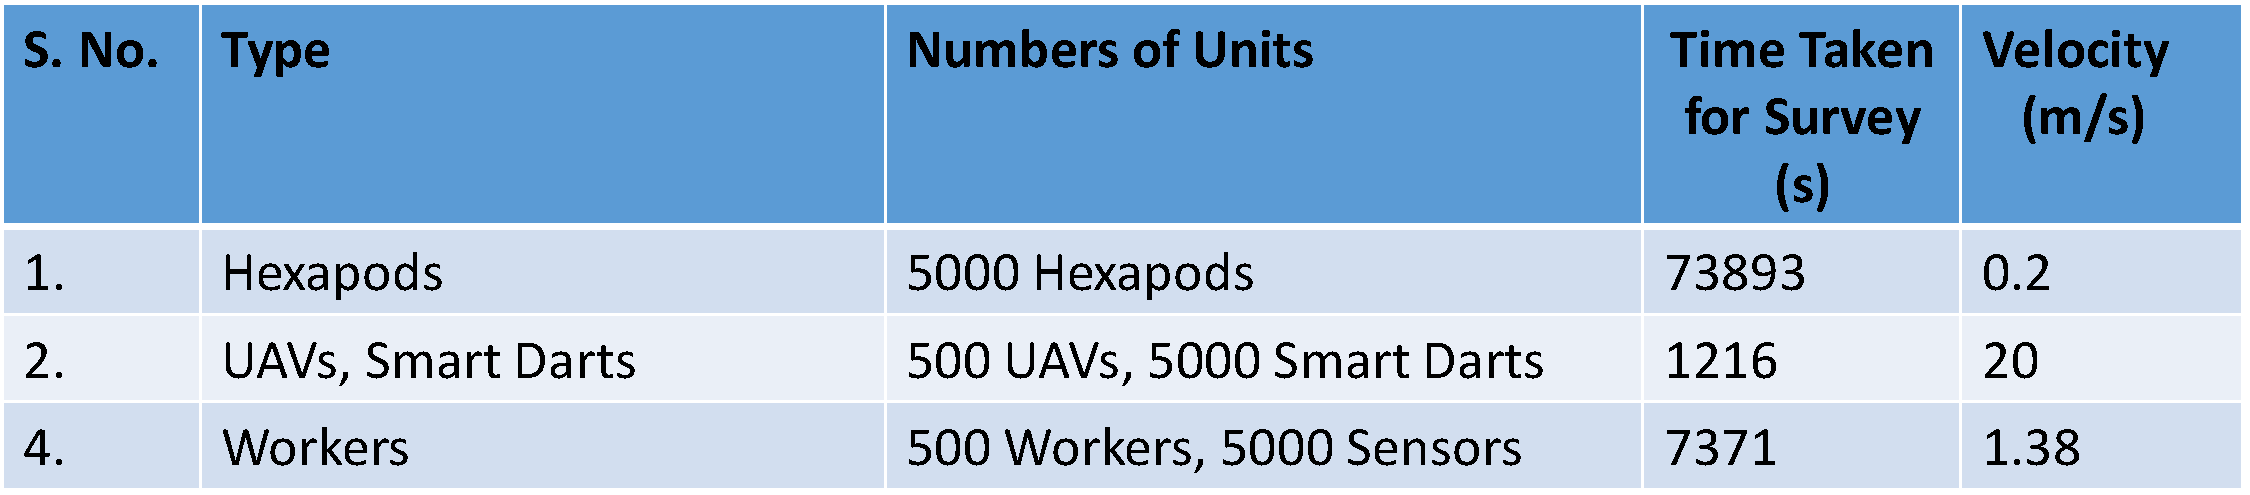
\includegraphics[width=\columnwidth]{simulation_table.pdf}}
 \caption{Comparison of different  deployment modes highlights the efficiency of UAV deployment.} 
 \label{tab:Sim_table}
\end{table}

\begin{figure} \centering
  {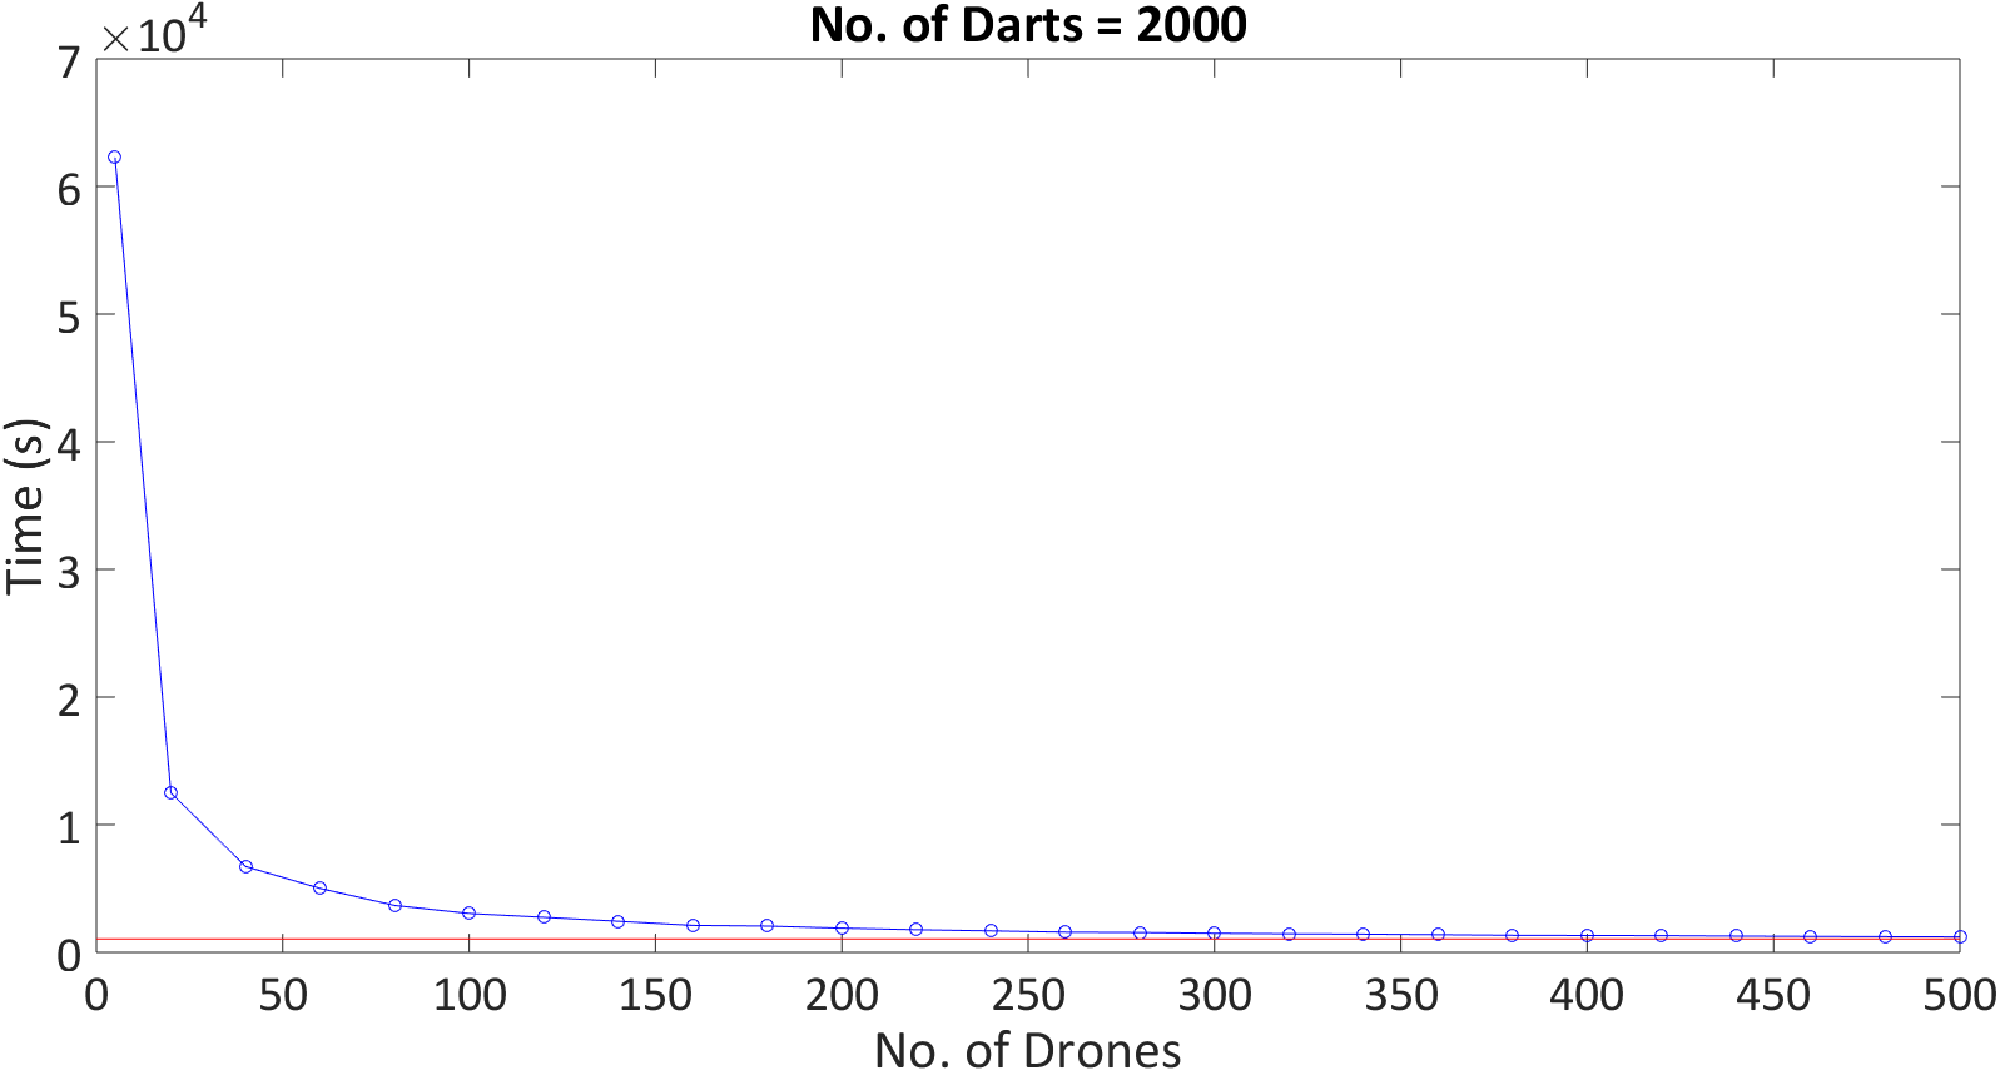
\includegraphics[width=\columnwidth]{DronevsTime.pdf}}
 \caption{Survey time for a 1km x 10 km region for different numbers of UAVs.} 
 \label{fig:DronevsTime}
\end{figure}

\begin{figure} \centering
  {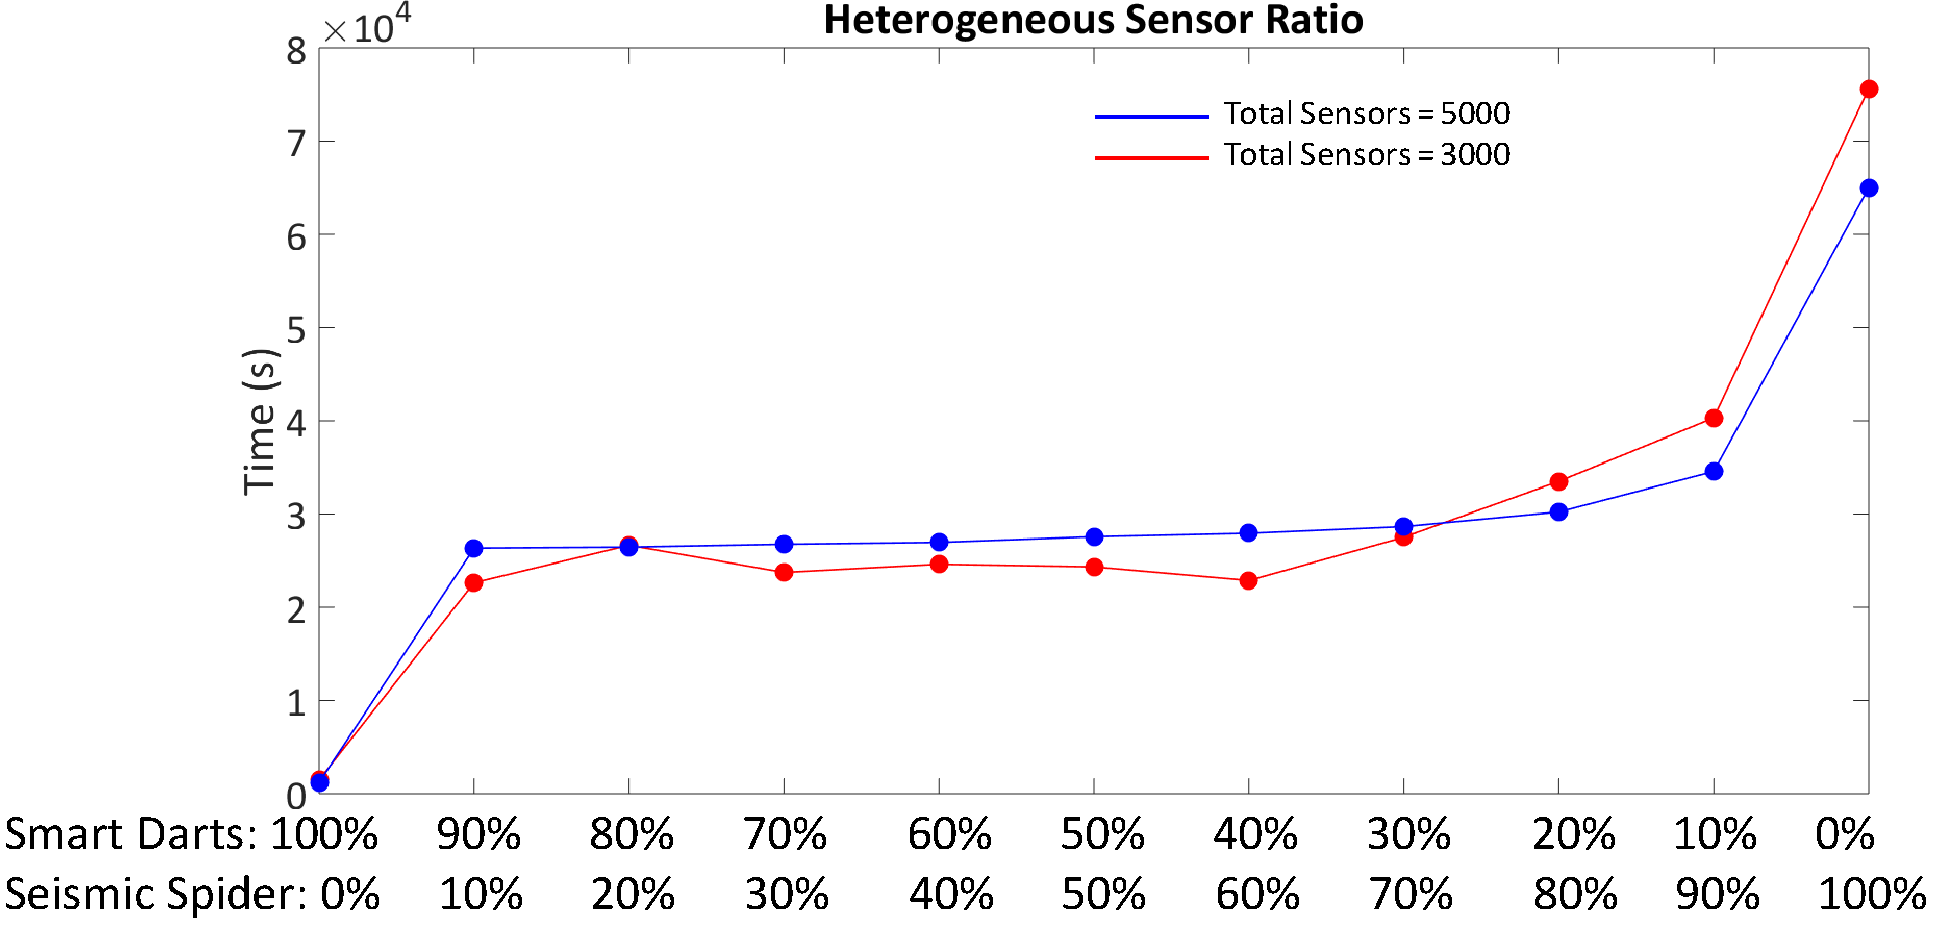
\includegraphics[width=\columnwidth]{het_sen_ratio.pdf}}
 \caption{Survey time for different sensor ratios. The total number of sensors \{5000, 3000\} were kept constant. Ten darts were provided for each UAV. } 
 \label{fig:het_sen_ratio}
\end{figure}

\subsection{Simulation Studies}


A scheduling system to compare  time and costs for seismic surveys with varying numbers of UAVs, SeismicSpiders, SeismicDarts, and human laborers was coded in  {\sc Matlab}, available at \cite{Srikanth2016seismicScheduler}. Frames from four different cases are shown in Fig.~\ref{fig:Sim_overview}.

This tool allows us to examine engineering and logistic trade-offs quickly in simulation.  For example, Fig.~\ref{fig:DronevsTime} assumes a fixed number of darts, and examines the finishing time with $5$ to $500$ UAVs.  The time required decays asymptotically, but $140$ UAVs requires only twice the amount of time required for $500$ UAVs, indicating that $140$ UAVs are sufficient for the task.    
 Substantial cost savings can be obtained by selecting the number of UAVs required to complete within a certain percentage greater than the optimal time.

The tool is useful for comparing the effectiveness of heterogeneous teams.  Table~\ref{tab:Sim_table} compares surveying a $1$ km x $10$ km strip of land with teams of (a) $5000$ SeismicSpiders, (b) $500$ UAVs and $5000$ SeismicDarts, (c) $500$ humans and $5000$ geophones.  Team (b) completed $6$ times faster than team (c). 
  Since SeismicSpiders are  slower than UAVs and humans, and are expensive compared to the SeismicDarts, their use is limited to special occasions. The Seismic UAV has the ability to deploy the SeismicSpider at a given waypoint. This attribute was not considered in the simulation but would improve deployment speed of SeismicSpiders.
   
In Fig.~\ref{fig:het_sen_ratio}, the total number of mobile agents are constant, but the percentage of UAVs and SeismicSpiders are varied. The goal is to analyze ratios of different sensors to optimize cost and time. 10 SeismicDarts were provided for each UAV. Increasing the percentage of UAVs lowers the deployment time. This is obvious since UAVs move at 20 m/s whereas SeismicSpiders move at 0.2 m/s. The difference in velocities makes UAV deployment time efficient. The SeismicSpiders are ideal for hard surface sensing or regions difficult for UAVs to access such as  forests.


%
 \section{Conclusion and Future Work}\label{sec:Conclusion}
This paper presented an autonomous technique for geophone placement, recording, and retrieval. The system enables automating a job that currently requires large teams of manual laborers. Three components were introduced, SeismicDarts, a mobile SeismicSpider, and a deployment unit.
Field and laboratory hardware experiments demonstrated the efficacy of the robotic team compared to traditional techniques. 
The SeismicDart's output were comparable to well-planted geophones. 
For hard surfaces where the SeismicDart could not penetrate, an autonomous alternative was presented, the SeismicSpider.  
The SeismicSpider is mobile, can actively adjust its sensors to ensure ground contact and vertical placement, and can be deployed and retrieved by UAVs.

Autonomous deployment was conducted using GPS, proving human involvement could be minimized by adopting the proposed technique. 
Hardware experiments compared the autonomous system to manual planting and ballistic deployment.
Simulation studies show time and cost savings over traditional manual techniques.

Future systems should be weatherized and optimized for cost, robustness, range, and speed. 



\bibliographystyle{IEEEtran}
\bibliography{./bibs/Match}

% that's all folks
\end{document}


